% arara: xelatex
\documentclass[handout, xcolor=dvipsnames]{beamer}
  \usepackage{eso-pic}
  \usepackage{lmodern}% http://ctan.org/pkg/lm
  \usepackage{fix-cm} % Fixes warnings about missing fonts; see http://tex.stackexchange.com/questions/32378/xfrac-siunitx-gives-me-a-font-warning
  \usepackage{stmaryrd}
  \usepackage{soul}
  \usepackage{amssymb,amsthm,amsmath,amsxtra}
  \usepackage[all]{xy}
  \usepackage{xfrac}
  \usepackage{calc}
  \usepackage{tikz}
  \usetikzlibrary{arrows,calc,automata,shadows,backgrounds,positioning,intersections,fadings,decorations.pathreplacing,shapes,snakes, matrix}
  \usepackage{tikz-cd}
  \tikzset{commutative diagrams/.cd, arrow style = tikz, diagrams = {>=latex}}
  \tikzset{>=latex}
  \usepackage{marvosym}
  \usepackage[marvosym]{tikzsymbols}
  \usepackage{beamerthemesplit}
  % \usecolortheme[named=SeaGreen]{structure}
  \definecolor{DartGreen}{cmyk}{0.95,0,1,0.50}
  % 95, 0, 100, 50
  \usecolortheme[named=DartGreen]{structure}
  % \usecolortheme[named=OliveGreen]{structure}
  % \usetheme{Singapore}
  % \setbeamersize{text margin top=-1in}
  \setbeamertemplate{navigation symbols}{}%remove navigation symbols
  \addtolength{\parskip}{0.5\baselineskip}
  \setlength{\arraycolsep}{2pt}
  \DeclareMathOperator{\AJ}{AJ}
  \DeclareMathOperator{\area}{area}
  \DeclareMathOperator{\opchar}{char}
  \DeclareMathOperator{\opdiv}{div}
  \DeclareMathOperator{\grad}{grad}
  \DeclareMathOperator{\Cl}{Cl}
  \DeclareMathOperator{\disc}{disc}
  \DeclareMathOperator{\Gal}{Gal}
  \DeclareMathOperator{\id}{id}
  \DeclareMathOperator{\M}{M}
  \DeclareMathOperator{\tr}{tr}
  \DeclareMathOperator{\nrd}{nrd}
  \DeclareMathOperator{\opP}{P}
  \DeclareMathOperator{\OO}{O}
  \DeclareMathOperator{\PGL}{PGL}
  \DeclareMathOperator{\GL}{GL}
  \DeclareMathOperator{\PSL}{PSL}
  \DeclareMathOperator{\PSU}{PSU}
  \DeclareMathOperator{\SL}{SL}
  \DeclareMathOperator{\SO}{SO}
  \DeclareMathOperator{\vol}{vol}
  \DeclareMathOperator{\Mon}{Mon}
  \DeclareMathOperator{\rad}{rad}
  \DeclareMathOperator{\Aut}{Aut}
  \newcommand{\quat}[2]{\displaystyle{\bigly(\frac{#1}{#2}\biggr)}}
  \theoremstyle{plain}
  \newtheorem*{thm}{Theorem}
  \newtheorem*{lem}{Lemma}
  \newtheorem*{prop}{Proposition}
  \newtheorem*{ques}{Question}
  \newtheorem*{conj}{Conjecture}
  \newtheorem*{cor}{Corollary}
  \newcommand{\psmod}[1]{~(\textup{\text{mod}}~{#1})}
  \newcommand{\CC}{\mathbb C}
  \newcommand{\A}{\mathbb A}
  \newcommand{\F}{\mathbb F}
  \newcommand{\HH}{\mathbb H}
  \newcommand{\PP}{\mathbb P}
  \newcommand{\R}{\mathbb R}
  \newcommand{\Q}{\mathbb Q}
  \newcommand{\Z}{\mathbb{Z}}
  \newcommand{\Qbar}{\overline{\mathbb Q}}
  \newcommand{\calD}{\mathcal{D}}
  \newcommand{\calG}{\mathcal{G}}
  \newcommand{\calH}{\mathcal H}
  \newcommand{\calO}{\mathcal O}
  \newcommand{\wt}[1]{\widetilde{#1}}
  \newcommand{\defi}[1]{\textbf{#1}} 				% for defined terms
  \setlength{\hfuzz}{4pt}
  % \newcommand{\Belyi}{Bely\u{\i}}
  \newcommand{\legen}[2]{\left(\frac{#1}{#2}\right)}

\title{$2$-Group Belyi Maps}
\author{Michael Musty}
\date{}

\newcommand\AtPagemyUpperLeft[1]{\AtPageLowerLeft{%
\put(\LenToUnit{0.87\paperwidth},\LenToUnit{0.815\paperheight}){#1}}}
\newcommand\AtPagemyLowerRight[1]{\AtPageLowerLeft{%
  \put(\LenToUnit{0.88\paperwidth},\LenToUnit{0.02\paperheight}){#1}}}
\AddToShipoutPictureFG{
  \AtPagemyUpperLeft{{
\includegraphics[scale=.081]{chseal-white.png}}}
  % \AtPagemyLowerRight{
  %   \usebeamerfont{framenumber}\insertframenumber{} / \inserttotalframenumber\hspace*{2ex}
  % }
}%

\begin{document}
  \begin{frame}[plain]
    \begin{center}{
      \Huge\color{DartGreen}
      $2$-Group
      Belyi Maps
    }
    \end{center}
    \begin{center}
      \only<1>{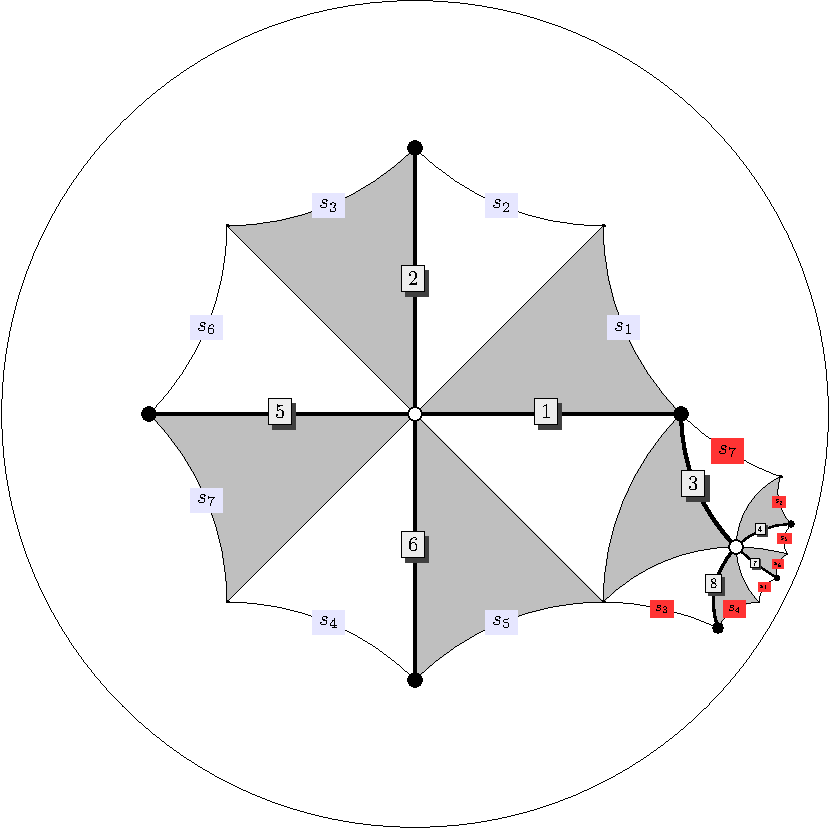
\includegraphics[scale = 0.3]{8T5-g2.pdf}}
      \only<2>{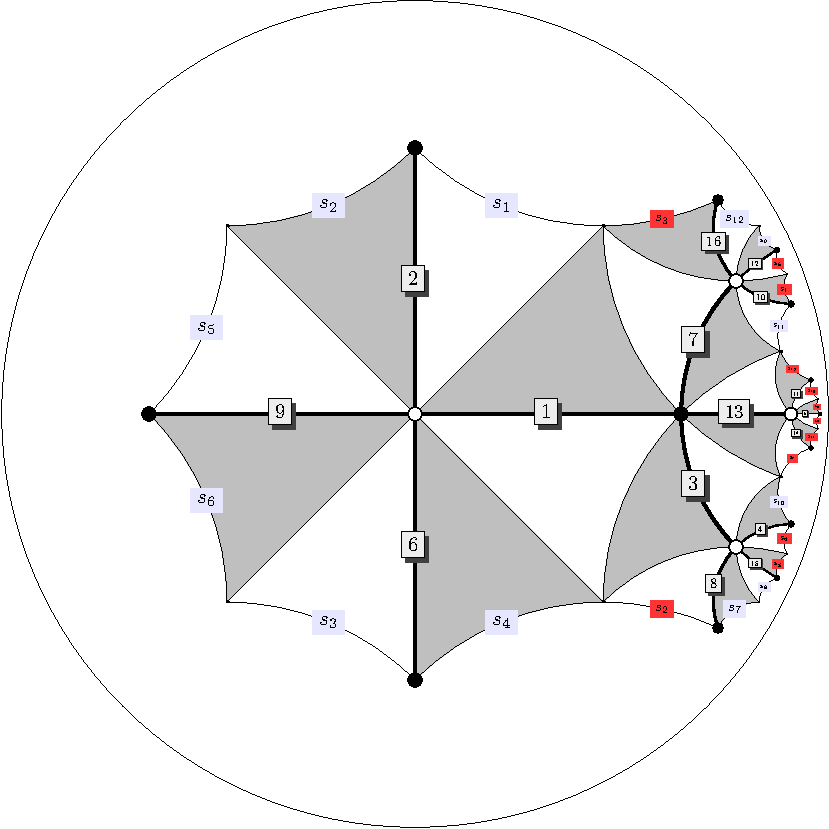
\includegraphics[scale = 0.3]{16T8-g3.pdf}}
      \only<3>{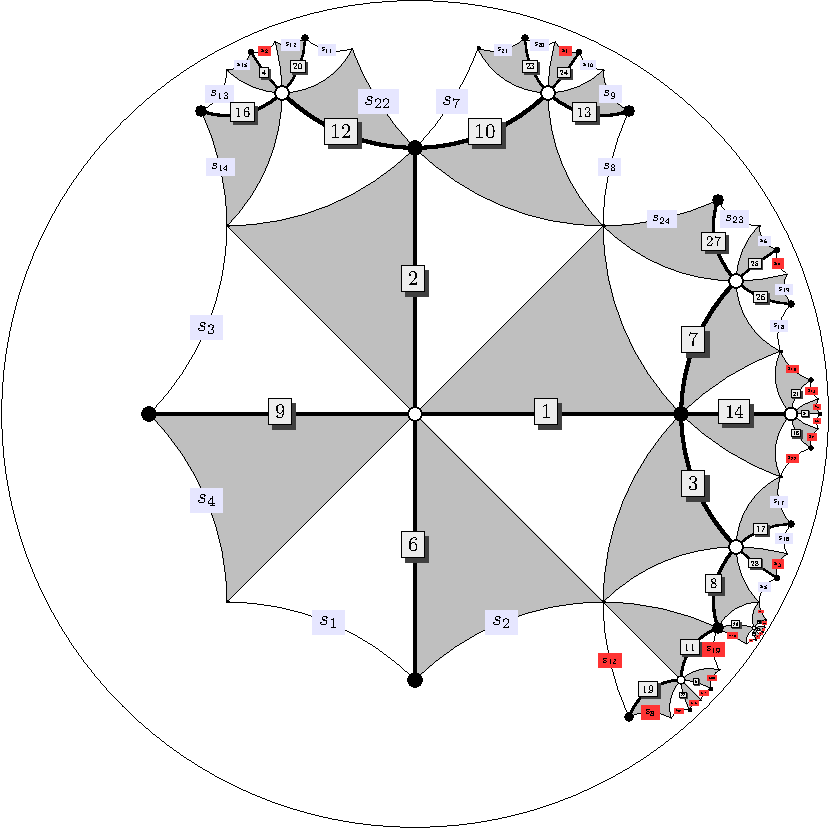
\includegraphics[scale = 0.3]{32S2-g5.pdf}}
      \only<4>{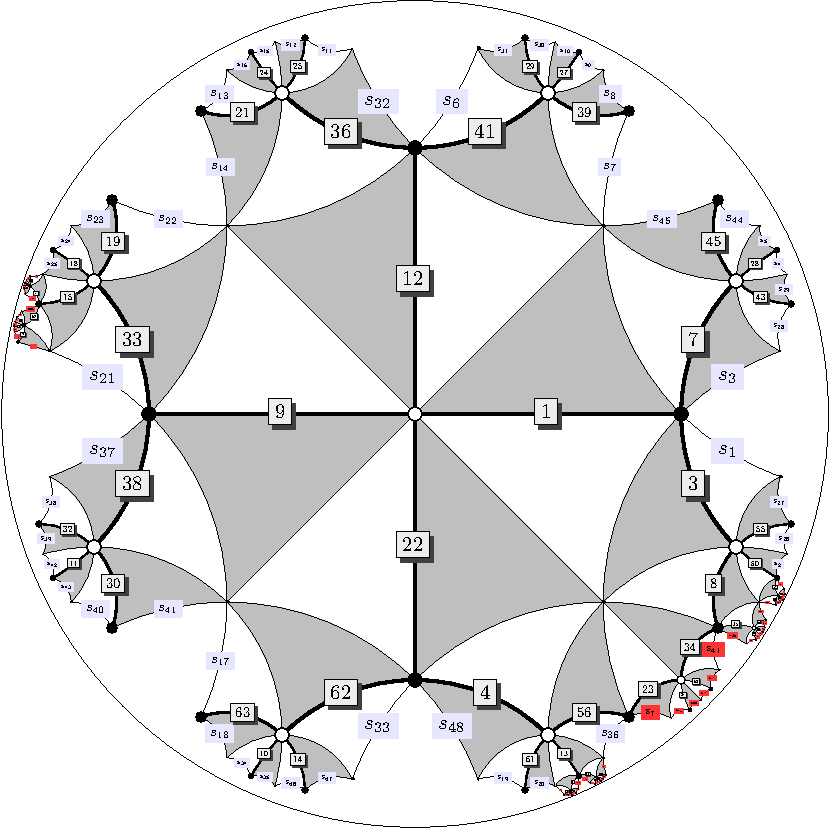
\includegraphics[scale = 0.3]{64S23-g9.pdf}}
      \only<5>{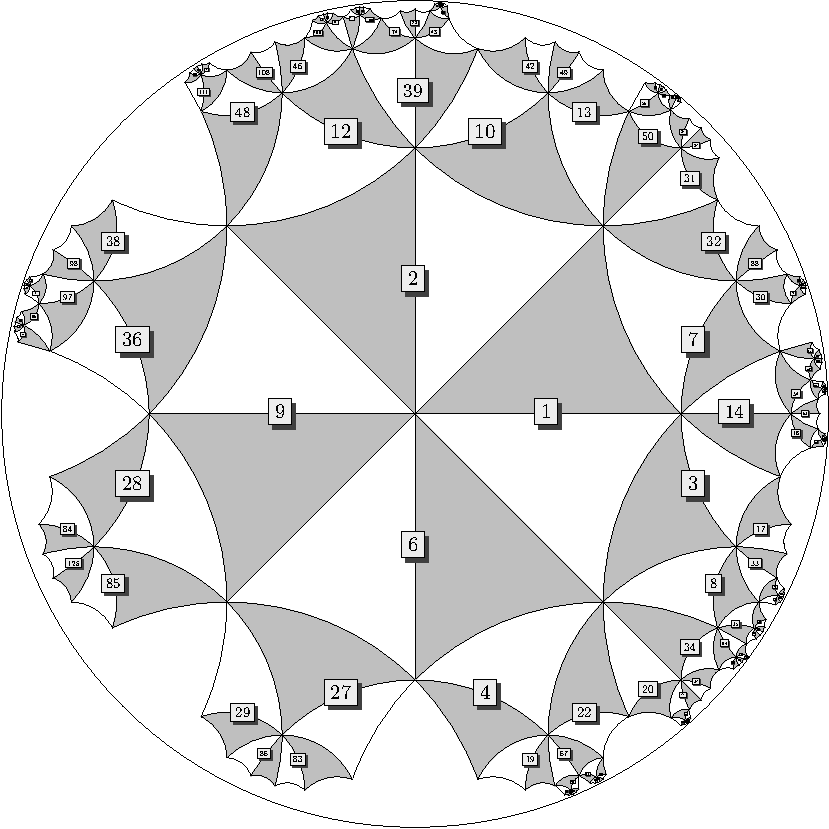
\includegraphics[scale = 0.3]{128S36-g17.pdf}}
    \end{center}
    \begin{center}
      Michael Musty\\
      % \url{https://michaelmusty.github.io/}\\
      \url{https://math.dartmouth.edu/~mjmusty}\\
      AMS Special Session on Number Theory, Arithmetic Geometry, and Computation\\
      January 19, 2019
    \end{center}
  \end{frame}
  % \begin{frame}[plain]
  %   \frametitle{Outline}
  %   \begin{itemize}
  %     \item
  %       Why $p=2$?
  %     \item
  %       What is a 2-Group Belyi map?
  %       \begin{itemize}
  %         \item
  %           Belyi's theorem
  %         \item
  %           Permutation triples
  %         \item
  %           Passports
  %         \item
  %           2-group Belyi maps and Beckmann's theorem
  %       \end{itemize}
  %     \item
  %       Computing all 2-group Belyi maps of a given degree
  %       \begin{itemize}
  %         \item
  %           Computing permutation triples
  %         \item
  %           Computing equations
  %       \end{itemize}
  %     \item
  %       By day and by night
  %   \end{itemize}
  % \end{frame}
  \begin{frame}[plain]
    \frametitle{Why $p=2$?}
    \begin{conj}[Gross 1998]
      For every prime $p$, there exists a nonsolvable Galois number field
      ramified only at $p$.
    \end{conj}
    \pause
    $p\geq 11$ : existence (Serre), explicit (Edixhoven, Mascot)
    \par
    $p=7$ : existence (Dieulefait)
    \par
    $p=5$ : existence (Demb\'{e}l\'{e}, Greenberg, Voight), explicit (Roberts)
    \par
    $p=3$ : existence (Demb\'{e}l\'{e}, Greenberg, Voight)
    \par
    $p=2$ : existence (Demb\'{e}l\'{e})
    \pause
    \par
    The hope is that an explicit nonsolvable field ramified only at $2$
    can be obtained from a $2$-group Belyi curve.
  \end{frame}
  % \begin{frame}[plain]
    % \frametitle{Motivation: Beckmann's Theorem}
    % \pause
    % \begin{thm}[Beckmann 1989]
    %   Let $\phi:X\to\PP^1$ be a Belyi map with monodromy group $G$.
    %   \pause
    %   Suppose $p$ does not divide $\#G$.
    %   \pause
    %   Then there exists a number field $M$ such that $p$
    %   is unramified in $M$ and
    %   \pause
    %   $\phi$ is defined over $M$ with good reduction at all
    %   primes $\mathfrak{p}$ of $M$ above $p$.
    % \end{thm}
    % \pause
    % \textbf{Upshot}:
    % \pause
    % Every $2$-group Belyi curve has a model with
    % good reduction away from $p=2$.
  % \end{frame}
  % \begin{frame}[plain]
    % \frametitle{Interesting number fields}
    % \pause
    % \begin{ques}
    %   \pause
    %   Is there a $2$-group Belyi curve whose Jacobian has a $2$-torsion field
    %   that is not solvable?
    % \end{ques}
  % \end{frame}
  \begin{frame}[plain]
    \frametitle{Belyi's Theorem}
    \begin{thm}[G.V. Belyi 1979]
      A smooth projective curve $X$ over $\CC$
      can be defined over $\overline{\Q}$ if and only if there
      exists a branched covering of compact connected Riemann surfaces $\phi:X\to\PP^1$
      unramified (unbranched) above $\PP^1\setminus\{0,1,\infty\}$.
    \end{thm}
    \pause
    Such a map is called a \textbf{Belyi map}.
    We will denote the \textbf{monodromy group} of a Belyi map $\phi$ by $\Mon(\phi)$.
    % Two Belyi maps $\phi:X\to\PP^1$ and $\phi':X'\to\PP^1$ are
    % \defi{isomorphic} if there is an isomorphism $\iota:X\to X'$
    % such that $\phi'\iota = \phi$.
  \end{frame}
  \begin{frame}[plain]
    \frametitle{Permutation Triples}
    A \textbf{transitive permutation triple of degree $d$} is a triple
    \[
      \sigma = (\sigma_0, \sigma_1, \sigma_\infty)\in S_d^3
    \]
    such that
    \begin{itemize}
      \item
        $\sigma_\infty\sigma_1\sigma_0=1$
      \item
        $\sigma$ generates a transitive subgroup of $S_d$
    \end{itemize}
    \pause
    The set of degree $d$ Belyi maps up to isomorphism is in bijection with the
    set of degree $d$ transitive permutation triples up to
    \textbf{simultaneous conjugation} and
    the group $\langle\sigma\rangle$ is the monodromy group of $\phi$.
  \end{frame}
  \begin{frame}[plain]
    \frametitle{Passports}
    A \textbf{passport} $\mathcal{P}$ consists of the data
    $(g,G,\lambda)$ where $g\geq 0$ is an integer,
    $G\leq S_d$ is a transitive subgroup,
    and $\lambda = (\lambda_0,\lambda_1,\lambda_\infty)$
    is a triple of partitions of $d$.
    \pause
    \par
    The \textbf{passport of a Belyi map} $\phi:X\to\PP^1$
    is $(g(X), \Mon(\phi), (\lambda_0,\lambda_1,\lambda_\infty))$
    with $g(X)$ the genus of $X$,
    $\Mon(\phi)$ the monodromy group of $\phi$,
    and the partitions specified by ramification.
    \pause
    \par
    The \textbf{passport of a permutation triple} $\sigma$ is
    $(g(\sigma), \langle\sigma\rangle, \lambda(\sigma))$
    where
    $$
    g(\sigma) = 1-d+(e(\sigma_0)-e(\sigma_1)-e(\sigma_\infty))/2
    $$
    with
    $$
    e(\tau) = d-\#\text{cycles of }\tau,
    $$
    and $\lambda(\sigma)$ is specified by cycle structures.
    % \pause
    % \par
    % The \textbf{size of a passport} $\mathcal{P}$ is the number of
    % simultaneous conjugacy classes of transitive permutation triples
    % with passport $\mathcal{P}$.
  \end{frame}
  \begin{frame}[plain]
    \frametitle{$2$-Group Belyi maps and Beckmann's Theorem}
    A \textbf{Galois Belyi map} is a degree $d$ Belyi map $\phi$
    with $\#\Mon(\phi) = d$.
    \pause
    \par
    A \textbf{$2$-group Belyi map} is a Galois Belyi map $\phi$
    with $\Mon(\phi)$ a $2$-group.
    \pause
    \begin{thm}[Beckmann 1989]
      Let $\phi:X\to\PP^1$ be a Belyi map with monodromy group $G$.
      Suppose $p$ does not divide $\#G$.
      Then there exists a number field $M$ such that $p$
      is unramified in $M$ and
      $\phi$ is defined over $M$ with good reduction at all
      primes $\mathfrak{p}$ of $M$ above $p$.
    \end{thm}
    \pause
    % \begin{cor}
    %   The $2$-torsion field of the Jacobian of a $2$-group Belyi curve
    %   is ramified only at $2$.
    % \end{cor}
    The upshot of Beckmann's theorem
    is that every $2$-group Belyi curve has a model with
    good reduction away from $p=2$.
  \end{frame}
  \begin{frame}[plain]
    \frametitle{$2$-Group Belyi maps}
    \begin{center}
      \begin{tikzpicture}[scale=0.3]
        \node at (0,0) (X0) {$X_1 = \PP^1$};
        \node [above left=of X0] (X1) {$X_2$};
        \node [above =of X1] (X2) {$X_3$};
        \node [above =of X2] (dots) {$\vdots$};
        \node [above =of dots] (Xr) {$X_r$};
        %\draw[<->] (X1) to node [above,rotate=-35] {$\sim$} node {} (X0);
        \draw[->] (X1) to node [below] {$2$} node {} (X0);
        \draw[->] (X2) to node [left] {$2$} node {} (X1);
        \draw[->, bend left] (X2) to node [below, left] {} node {} (X0);
        \draw[->] (dots) to node [left] {$2$} node {} (X2);
        \draw[->] (Xr) to node [left] {$2$} node {} (dots);
        \draw[->, bend left] (Xr) to node [below, left] {} node {} (X0);
        %\node at (8,0) (KX0) {$K(X_1) = K(\PP^1)$};
        %\node [above left=of KX0] (KX1) {$K(X_2)$};
        %\node [above =of KX1] (KX2) {$K(X_3)$};
        %\node [above =of KX2] (dots) {$\vdots$};
        %\node [above =of dots] (KXr) {$K(X_r)$};
        %%\draw[<->] (X1) to node [above,rotate=-35] {$\sim$} node {} (X0);
        %\draw[-] (KX1) to node [below] {$2$} node {} (KX0);
        %\draw[-] (KX2) to node [left] {$2$} node {} (KX1);
        %\draw[-, bend left] (KX2) to node [below, left] {} node {} (KX0);
        %\draw[-] (dots) to node [left] {$2$} node {} (KX2);
        %\draw[-] (KXr) to node [left] {$2$} node {} (dots);
        %\draw[-, bend left] (KXr) to node [below, left] {} node {} (KX0);
      \end{tikzpicture}
    \end{center}
  \end{frame}
  \begin{frame}[plain]
    \frametitle{Computing $2$-group permutation triples}
    Let $\phi:X\to\PP^1$ be a Belyi map
    of degree $d = 2^\ell$
    corresponding
    \newline
    to $\sigma\in S_d^3$.
    \pause
    We want to find $\wt{\phi}:\wt{X}\to\PP^1$ corresponding
    to $\wt{\sigma}\in S_{2d}^3$ such that
    \[
      \begin{tikzcd}[ampersand replacement=\&]
        \widetilde{X}\arrow{dd}[swap]{\widetilde{\phi}}\arrow{dr}{2}\\
        \&X\arrow{dl}{\phi}\\
        \PP^1
      \end{tikzcd}
    \]
    \pause
    Such a $\wt{\sigma}$ sits in the following exact sequence of groups:
    \[
      \begin{tikzcd}[ampersand replacement=\&, row sep = small]
        1\arrow{r}\&\Z/2\Z\arrow{r}{\iota}\&\langle\widetilde{\sigma}\rangle\arrow{r}{\pi}\&\langle\sigma\rangle\arrow{r}\&1
      \end{tikzcd}
    \]
    Without loss of generality we can restrict our attention to
    \emph{central} extensions.
  \end{frame}
  \begin{frame}[plain]
    \frametitle{Computing $2$-group permutation triples}
    Let $\sigma$ correspond to a $2$-group Belyi map $\phi$.
    \begin{itemize}
      \item
        \pause
        \par
        Compute all equivalence classes of (central) extensions
        \[
          \begin{tikzcd}[ampersand replacement=\&, row sep = small]
            1\arrow{r}\&\Z/2\Z\arrow{r}{\iota}\&E\arrow{r}{\pi}\&\langle\sigma\rangle\arrow{r}\&1
          \end{tikzcd}
        \]
        The main tool used here is Derek Holt's
        algorithm to compute the second cohomology group
        of a finite group.
      \item
        \par
        \pause
        For each extension, we get $8$ possible $\wt{\sigma}$.
        We then check the necessary conditions for $\wt{\sigma}$ to
        correspond to a Belyi map to obtain all possible lifts of $\sigma$.
    \end{itemize}
  \end{frame}
  \begin{frame}[plain]
    \frametitle{Passport counts}
    \begin{thm}
      The following table lists the number of passports of
      $2$-group Belyi maps of degree $d$ for $d$ up to $256$.
      \[
        \begin{tabular}{|c||c|c|c|c|c|c|c|c|}
          \hline
          $d$ & $2$ & $4$ & $8$ & $16$ & $32$ & $64$ & $128$ & $256$\\
          \hline
          \# passports & $3$ & $7$ & $16$ & $41$ & $96$ & $267$ & $834$ & $2893$\\
          \hline
        \end{tabular}
      \]
    \end{thm}
  \end{frame}
  \begin{frame}[plain]
    \frametitle{Computing $2$-group Belyi maps}
    Let $\phi:X\to\PP^1$ be a Belyi map
    of degree $d = 2^\ell$
    corresponding
    \newline
    to $\sigma\in S_d^3$.
    \pause
    Given a permutation triple $\wt{\sigma}$ with
    \[
      \begin{tikzcd}[ampersand replacement=\&, row sep = small]
        1\arrow{r}\&\Z/2\Z\arrow{r}{\iota}\&\langle\widetilde{\sigma}\rangle\arrow{r}{\pi}\&\langle\sigma\rangle\arrow{r}\&1
      \end{tikzcd},
    \]
    let us now consider the problem of finding the Belyi map
    corresponding to $\wt{\sigma}$.
    \pause
    Let $X\subseteq\A_K^n$ with defining equations
    $\{g_i\}_{i=1}^s\subset K[x_1,\dots,x_n]$.
    \pause
    Our goal is to find $f\in K(X)^\times$ such that
    \[
      \begin{tikzcd}[ampersand replacement=\&]
        \widetilde{X}\arrow{dd}[swap]{\widetilde{\phi}}\arrow{dr}{\psi}\\
        \&X\arrow{dl}{\phi}\\
        \PP^1
      \end{tikzcd}
      \quad
      \quad
      \quad
      \begin{tikzcd}[ampersand replacement=\&]
        \frac{\overline{K}(X)[y]}{(y^2-f)}\arrow[dash]{dd}\arrow[dash]{dr}{2}\\
        \&\overline{K}(X)\arrow[dash]{dl}{d}\\
        \overline{K}(\PP^1)
      \end{tikzcd}
    \]
    with $\psi$ (and hence $\wt{\phi}$) satisfying the ramification conditions imposed by
    $\wt{\sigma}$.
  \end{frame}
  \begin{frame}[plain]
    \frametitle{Computing $2$-group Belyi maps}
    The procedure to find $f\in K(X)$ is as follows:
    \begin{enumerate}
      \pause
      \item
        Let $\{Q_i\}$ be the points on $X$ that we want to
        be ramification values of $\psi$.
        These are determined by $\wt{\sigma}$.
      \item
        Build a degree $0$ divisor $D = \sum_{P} n_P P$
        with $n_{Q_i}$ odd for every $i$.
      \item
        Try to find $f$ in the (computable) Riemann-Roch space $L(D)$.
    \end{enumerate}
    \pause
    There are (at least) two remarks to make about this process:
    \begin{itemize}
      \item
        Extending the base field $K$ may be necessary
        to determine $D$.
      \item
        Class group obstruction.
    \end{itemize}
  \end{frame}
  \begin{frame}[plain]
    \frametitle{Degree $4$ example}
    \begin{align*}
      \wt{\sigma}= \Big((1\,4\,3\,2),(1\,3)(2\,4),(1\,4\,3\,2)\Big),
      \quad
      \sigma= \Big((1\,2),(1)(2),(1\,2)\Big)
    \end{align*}
    \begin{tikzpicture}[scale=.5]
      %\draw[thin,gray] (-20,-1) grid (20,5);
      % Y1 to Y0
      % affine curves
      \node (Y0) at (0,0) {$X_1$};
      \node (Y1) at (-4,5) {$X_2:x_2^2=x_1$};
      %\node (Y2) at (-4,10) {$X_3:\substack{x_2^2=x_1\\x_3^2=x_2^3-x_2}$};
      % maps of affine curves
      %\draw[->] (Y1)--(Y0) node [pos=.5,left] {$(x_0,x_1)\mapsto x_0=x_1^2$};
      \draw[->] (Y1)--(Y0);
      %\draw[->] (Y2)--(Y1) node [pos=.5,left] {$(x_0,x_1)$};
      %\draw[->] (Y2)--(Y1);
      %\draw[->,thick,blue,bend left] (Y2) to node [pos=.25,right] {$x_0 = x_1^2$} (Y0);
      %\draw[->,thick,bend left] (Y2) to (Y0);
      % function fields
      \node (KX0) at (20,0) {$K(X_0) = K(x_0)$};
      \node (KX1) at (16,5) {$K(X_1) = \frac{K(x_0)[x_1]}{\left(x_1^2-x_0\right)}$};
      %\node (KX2) at (16,10) {$K(X_2) = \frac{K(X_1)[x_2]}{\left(x_2^2-(x_1^3-x_1)\right)}$};
      \draw[->] (KX0) to (KX1);
      %\draw[->] (KX1) to (KX2);
      %\draw[->,thick,blue,bend right] (KX0) to (KX2);
      % ramification
      \node (Y0 0) at (-20,0) {$0$};
      \node (Y0 1) at (-15,0) {$1$};
      \node (Y0 oo) at (-10,0) {$\infty$};
      \node (Y1 0) at (-20,5) {$(0,0)$};
      \node (Y1 1) at (-20+10/3,5) {$(1,1)$};
      \node (Y1 -1) at (-20+20/3,5) {$(1,-1)$};
      \node (Y1 oo) at (-10,5) {$\infty$};
      %\node (Y2 0) at (-20,10) {$(0,0,0)$};
      %\node (Y2 1) at (-20+10/3,10) {$(1,1,0)$};
      %\node (Y2 -1) at (-20+20/3,10) {$(1,-1,0)$};
      %\node (Y2 oo) at (-10,10) {$\infty$};
      \draw[double distance=1pt] (Y1 0) to (Y0 0);
      \draw (Y0 1) to (Y1 1);
      \draw (Y1 -1) to (Y0 1);
      \draw[double distance=1pt] (Y1 oo) to (Y0 oo);
      %\draw[double distance=1pt] (Y2 0) to (Y1 0);
      %\draw[double distance=1pt] (Y2 1) to (Y1 1);
      %\draw[double distance=1pt] (Y2 -1) to (Y1 -1);
      %\draw[double distance=1pt] (Y2 oo) to (Y1 oo);
    \end{tikzpicture}
  \end{frame}
  \begin{frame}[plain]
    \frametitle{Degree $4$ example}
    \begin{align*}
      \wt{\sigma}= \Big((1\,4\,3\,2),(1\,3)(2\,4),(1\,4\,3\,2)\Big),
      \quad
      \sigma= \Big((1\,2),(1)(2),(1\,2)\Big)
    \end{align*}
    \begin{tikzpicture}[scale=.5]
      %\draw[thin,gray] (-20,-1) grid (20,5);
      % Y1 to Y0
      % affine curves
      \node (Y0) at (0,0) {$X_1$};
      \node (Y1) at (-4,5) {$X_2:x_2^2=x_1$};
      \node (Y2) at (-4,10) {$X_3:\substack{x_2^2=x_1\\x_3^2=x_2^3-x_2}$};
      % maps of affine curves
      %\draw[->] (Y1)--(Y0) node [pos=.5,left] {$(x_0,x_1)\mapsto x_0=x_1^2$};
      \draw[->] (Y1)--(Y0);
      %\draw[->] (Y2)--(Y1) node [pos=.5,left] {$(x_0,x_1)$};
      \draw[->] (Y2)--(Y1);
      %\draw[->,thick,blue,bend left] (Y2) to node [pos=.25,right] {$x_0 = x_1^2$} (Y0);
      \draw[->,thick,bend left] (Y2) to (Y0);
      % function fields
      \node (KX0) at (20,0) {$K(X_0) = K(x_0)$};
      \node (KX1) at (16,5) {$K(X_1) = \frac{K(x_0)[x_1]}{\left(x_1^2-x_0\right)}$};
      \node (KX2) at (16,10) {$K(X_2) = \frac{K(X_1)[x_2]}{\left(x_2^2-(x_1^3-x_1)\right)}$};
      \draw[->] (KX0) to (KX1);
      \draw[->] (KX1) to (KX2);
      \draw[->,thick,blue,bend right] (KX0) to (KX2);
      % ramification
      \node (Y0 0) at (-20,0) {$0$};
      \node (Y0 1) at (-15,0) {$1$};
      \node (Y0 oo) at (-10,0) {$\infty$};
      \node (Y1 0) at (-20,5) {$(0,0)$};
      \node (Y1 1) at (-20+10/3,5) {$(1,1)$};
      \node (Y1 -1) at (-20+20/3,5) {$(1,-1)$};
      \node (Y1 oo) at (-10,5) {$\infty$};
      \node (Y2 0) at (-20,10) {$(0,0,0)$};
      \node (Y2 1) at (-20+10/3,10) {$(1,1,0)$};
      \node (Y2 -1) at (-20+20/3,10) {$(1,-1,0)$};
      \node (Y2 oo) at (-10,10) {$\infty$};
      \draw[double distance=1pt] (Y1 0) to (Y0 0);
      \draw (Y0 1) to (Y1 1);
      \draw (Y1 -1) to (Y0 1);
      \draw[double distance=1pt] (Y1 oo) to (Y0 oo);
      \draw[double distance=1pt] (Y2 0) to (Y1 0);
      \draw[double distance=1pt] (Y2 1) to (Y1 1);
      \draw[double distance=1pt] (Y2 -1) to (Y1 -1);
      \draw[double distance=1pt] (Y2 oo) to (Y1 oo);
    \end{tikzpicture}
  \end{frame}
  \begin{frame}[plain]
    \frametitle{A refined conjecture (by day)}
    A \textbf{refined passport} $\mathcal{P}$ consists of the data
    $(g,G,C)$
    \newline
    where $g\geq 0$ is an integer,
    $G\leq S_d$ is a transitive subgroup,
    and $C = (C_0,C_1,C_\infty)$
    is a triple of conjugacy classes of $G$.
    \par
    \pause
    For a refined passport $\mathcal{P}$ consider the set
    % \[
    %   \Sigma_\mathcal{P} =
    %   \frac{\{(\sigma_0,\sigma_1,\sigma_\infty)\in C_0\times C_1\times C_\infty : \sigma_\infty\sigma_1\sigma_0=1,\text{ and } \langle\sigma\rangle=G\}}{\sim}
    % \]
    \[
      \Sigma_\mathcal{P} =
      \{(\sigma_0,\sigma_1,\sigma_\infty)\in C_0\times C_1\times C_\infty : \sigma_\infty\sigma_1\sigma_0=1,\text{ and } \langle\sigma\rangle=G\}/\sim
    \]
    where $(\sigma_0,\sigma_1,\sigma_\infty)\sim(\sigma_0', \sigma_1', \sigma_\infty')$
    if and only if there exists $\alpha\in\Aut(G)$ with
    $\alpha(\sigma_s) = \sigma_s'$ for $s\in\{0,1,\infty\}$.
    \pause
    \begin{conj}
      Let $\mathcal{P} = (g,G,C)$
      be a refined passport with
      $G=\Mon(\phi)$ for some $2$-group Belyi map $\phi$.
      Then $\#\Sigma_\mathcal{P} = 0\text{ or }1$.
    \end{conj}
    \pause
    \begin{cor}
      Every $2$-group Belyi map is defined over a cyclotomic field
      $\Q(\zeta_{2^m})$ for some $m$.
    \end{cor}
  \end{frame}
  \begin{frame}[plain]
    \frametitle{Searching for a nonsolvable field (by night)}
    Let $X$ be a $2$-group Belyi curve
    defined over a field $K$
    with \newline Jacobian $A$.
    The hope is that $K(A[2])$ will be nonsolvable.
    \par
    How to compute $K(A[2])$ given $X$?
    \begin{itemize}
      \item
        Sage (Bruin, Sijsling)
      \item
        Sage/Magma (Costa, Mascot, Sijsling, Voight)
      \item
        Magma (Neurohr)
      \item
        Pari/gp (Mascot)
    \end{itemize}
    \par
    Which curve?
    \begin{itemize}
      \item
        Coarse factorizations of $A$ (Paulhus)
      \item
        Compute $\Aut(X)$ exploiting $2$-group structure
      \item
        Consider Belyi maps that are not Galois?
    \end{itemize}
    \pause
    Thanks for listening!
  \end{frame}
  % \begin{frame}[plain]
  %   \frametitle{Analyzing the data}
  %   \url{https://dessin-explorer.org}
  % \end{frame}
  % \begin{frame}[plain]
  %   \frametitle{Acknowledgements}
  %   Thanks to
  %   Sam Schiavone, Jeroen Sijsling, and John Voight
  %   for helpful conversations.
  %   \par
  %   {
  %     \Huge
  %     Thanks for listening!
  %   }
  % \end{frame}

%%%%%%%%%%%%%%%%%%%%%%%%%%%%%%%%%%%%%%%%%%%%%%%%%%%%%%%%%%%%%%%%%%%%%%%%%%%%%%%%
% OLD
%%%%%%%%%%%%%%%%%%%%%%%%%%%%%%%%%%%%%%%%%%%%%%%%%%%%%%%%%%%%%%%%%%%%%%%%%%%%%%%%

  %\begin{frame}[plain]
  %  \frametitle{Hyperelliptic Belyi maps}
  %  \pause
  %  Passport: \texttt{8T1-8,4,8-g3}, size 2
  %  % path1
  %  \newline
  %  Belyi curve: $X: y^2+(x^4+1)y=-2x^4$
  %  \newline
  %  Belyi map: $(y+1)^2$
  %  \pause
  %  \par
  %  Passport: \texttt{16T1-16,8,16-g7}, size 4
  %  % path1
  %  \newline
  %  Belyi curve: $X: y^2+(x^8+1)y=-2x^8$
  %  \newline
  %  Belyi map: $(y+1)^2$
  %\end{frame}
  %\begin{frame}[plain]
  %  \frametitle{Nonhyperelliptic Belyi maps}
  %  \pause
  %  \texttt{128S1-128,32,128-g62}
  %  $\to$
  %  \texttt{64S1-64,16,64-g30}
  %  $\to$
  %  \texttt{32S1-32,8,32-g14}
  %  $\to$
  %  \texttt{16T1-16,4,16-g6}
  %  $\to$
  %  \texttt{8T1-8,2,8-g2}
  %  $\to$
  %  \texttt{4T1-4,1,4-g0}
  %  $\to$
  %  \texttt{2T1-2,1,2-g0}
  %  \pause
  %  \begin{align*}
  %    X\subset\A^6:\;&x_1^5-x_1-x_2^2\\
  %       &x_1-x_1^3+x_2x_4^4\\
  %       &x_1^3x_3-x_1x_3-x_2x_4^2\\
  %       &x_1^2x_4^2-x_2x_3+x_4^2\\
  %       &x_2x_3-x_1^2-1\\
  %       &x_3x_4^2-1\\
  %       &x_5^2-x_4\\
  %       &x_6^2-x_5\\
  %    \phi:\;&x_3^4x_2^2-2x_3^2x_2+1
  %  \end{align*}
  %\end{frame}
  %\begin{frame}[plain]
  %  \frametitle{Nonhyperelliptic Belyi maps}
  %  % another noncyclic example
  %  \texttt{128S69-8,16,16-g49}: size 4
  %  \newline
  %  \texttt{64S7-4,8,8-g17}
  %  \newline
  %  \texttt{32S10-4,8,4-g7}
  %  \newline
  %  \texttt{16T12-4,8,2-g2}
  %  \newline
  %  \texttt{8T4-2,4,2-g0}
  %  \newline
  %  \texttt{4T2-2,2,2-g0}
  %  \newline
  %  \texttt{2T1-2,2,1-g0}
  %\end{frame}
  %\begin{frame}[plain]
  %  \frametitle{Networks?}
  %  \pause
  %  \url{https://math.dartmouth.edu/~mjmusty/32.html}
  %  \begin{itemize}
  %    \pause
  %    \item
  %      Is every $2$-group Belyi map defined over an abelian extension of $\Q$?
  %    \pause
  %    \item
  %      What can we say in the hyperelliptic case?
  %    \pause
  %    \item
  %      What infinite families of $2$-groups appear as monodromy groups of Belyi maps?
  %  \end{itemize}
  %  % abelian extensions for base fields
  %  % hyperelliptic not interesting
  %\end{frame}
  %\begin{frame}[plain]
  %  \frametitle{Acknowledgements}
  %  Thanks to the following for helpful discussions:
  %  \begin{itemize}
  %    \item Sam Schiavone
  %    \item Jeroen Sijsling
  %    \item John Voight
  %  \end{itemize}
  %  \pause
  %  Thanks for listening!
  %  \pause
  %  (unless there is extra time...)
  %\end{frame}
  %\begin{frame}[plain]
  %  \frametitle{Applications?}
  %  \pause
  %  Let $X$ be a $2$-group Belyi curve of degree $d$
  %  and genus $g$ defined over $K$.
  %  \pause
  %  We would like to compute the 2-torsion field of the jacobian $J$ of $X$.
  %  \pause
  %  The field $K(J[2])/K$ will be ramified only at $2$.
  %  \pause
  %  To start, we musty compute a period matrix for $J$.
  %  \pause
  %  We can embed $X$ in $\PP^2$ with a singular model.
  %  \pause
  %  Now consider an affine patch $f(x,y) = 0$.
  %  \pause
  %  The space of holomorphic $1$-forms on $X$
  %  is a subspace of
  %  \begin{align*}
  %    \left\{
  %      \frac{x^iy^j\;dx}{\partial_y f(x,y)} : 0\leq i,j\quad\text{and}\quad i+j\leq d-3
  %    \right\}
  %  \end{align*}
  %  \pause
  %  In some cases
  %  the exact space is given by $(i,j)$ where $(i+1,j+1)$
  %  is an interior point of the Newton polygon of $f(x,y)$.
  %  \pause
  %  (Baker 1893).
  %  \pause
  %  In general one must compute the adjoint ideal.
  %  \pause
  %  The next piece we need is a basis in homology.
  %  \pause
  %  Integrating yields a $g\times 2g$ period matrix $\Pi$
  %  \pause
  %  with $\Lambda$ the $\Z$-span of the columns of $\Pi$.
  %  \pause
  %  $J$ is identified with $\CC^g/\Lambda$.
  %\end{frame}
  %\begin{frame}[plain]
  %  \frametitle{Applications?}
  %  \pause
  %  The next piece is the Abel-Jacobi map
  %  \pause
  %  \begin{align*}
  %    \AJ:X&\to\CC^g/\Lambda\\
  %    P&\mapsto\left(\int_{P_0}^P\omega_j\right)_{j=1,\dots,g}
  %  \end{align*}
  %  \pause
  %  Now for $t\in\frac{1}{2}\Lambda/\Lambda$,
  %  \pause
  %  our task is to find $\{Q_1,\dots,Q_g\}$ with $Q_j\in X(\overline{K})$
  %  such that
  %  \pause
  %  \[
  %    \sum_{j=1}^g\left(\int_{P_0}^{Q_j}\omega_i\right)_{i=1,\dots,g}
  %  \]
  %  \pause
  %  The coordinates of the $Q_j$ generate the field $K(J[2])$.
  %\end{frame}
\end{document}
